In p-multigrid, the different grids have the same number and size of finite elements but with different order basis functions.
The grid transfer operators can be represented elementwise and can thus be easily represented in the form of Equation \ref{eq:libceed_representation}.

The prolongation operator from the coarse to the fine grid interpolates low-order basis functions at the nodes for the high-order basis functions.
Figure \ref{fig:p_prolongation} shows the evaluation of second order basis function on the Gauss-Lobatto nodes for a fourth order basis.
This basis evaluation operation will be extended for LFA of h-multigrid and BDDC.

\begin{figure}[!ht]
  \centering
  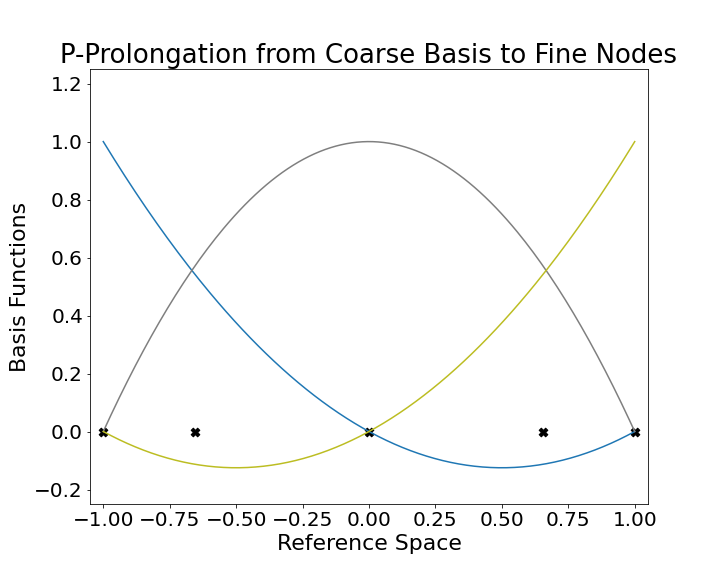
\includegraphics[width=0.48\textwidth]{../img/pProlongation}
  \caption{P-Prolongation from Coarse Basis to Fine Basis Points}
  \label{fig:p_prolongation}
\end{figure}

With this coarse to fine basis interpolation, the prolongation operator can be be represented by
\begin{equation}
\begin{tabular}{c}
${\color{burgundy}\mathbf{P}}_{\text{ctof}} = \mathbf{P}_f^T \mathbf{G}_f^T {\color{burgundy}\mathbf{P}}_e \mathbf{G}_c \mathbf{P}_c$\\
${\color{burgundy}\mathbf{P}}_e = {\color{blue(ncs)}\mathbf{I}} {\color{applegreen}\mathbf{D}}_{\text{scale}} {\color{blue(ncs)}\mathbf{B}}_{\text{ctof}}$
\end{tabular}
\end{equation}
where ${\color{blue(ncs)}\mathbf{B}}_{\text{ctof}}$ is an interpolation operator from the coarse grid basis to the fine grid basis, $\mathbf{P}_f$ and $\mathbf{G}_f$ are the fine grid element assembly operators, $\mathbf{P}_c$ and $\mathbf{G}_c$ are the coarse grid element assembly operators, and ${\color{applegreen}\mathbf{D}}_{\text{scale}}$ is a scaling operator to account for node multiplicity across element interfaces.
Restriction from the fine grid to the coarse grid is given by the transpose, ${\color{burgundy}\mathbf{R}}_{\text{ftoc}} = {\color{burgundy}\mathbf{P}}_{\text{ctof}}^T$.

It is useful to think of the p-prolongation operation as an interpolation operation between the coarse and fine grids, but in practice it can be easier to construct the prolongation basis ${\color{blue(ncs)}\mathbf{B}}_{\text{ctof}}$ from the coarse and fine grid interpolation operators, provided that both bases use the same quadrature space.
\begin{equation}
\begin{tabular}{c c}
${\color{blue(ncs)}\mathbf{B}}_f = \mathbf{Q} \mathbf{R},$ & ${\color{blue(ncs)}\mathbf{B}}_{\text{ctof}} = \mathbf{R}^{-1} \mathbf{Q}^T {\color{blue(ncs)}\mathbf{B}}_c$
\end{tabular}
\label{eq:p_prolong_basis}
\end{equation}
In Equation \ref{eq:p_prolong_basis}, we form the interpolation operation between the coarse grid from the coarse grid interpolation operator and the QR factorization of the fine grid interpolation operator.
Note that in the case of H1 Lagrange bases, this factorization will produce the same coarse to fine grid interpolation operator as evaluating the coarse grid basis functions at the fine grid nodes.

Following the derivation from Section \ref{sec:lfahighorder}, we can derive the symbols of ${\color{burgundy}\mathbf{P}}_{\text{ctof}}$ and ${\color{burgundy}\mathbf{R}}_{\text{ftoc}}$.

\begin{definition}
The symbol of the p-prolongation operator is given by
\begin{equation}
\tilde{{\color{burgundy}\mathbf{P}}}_{\text{ctof}} \left( \boldsymbol{\theta} \right) = \mathbf{Q}_f^T \left( {\color{burgundy}\mathbf{P}}_e \odot \left[ e^{\imath \left( \mathbf{x}_{j, c} - \mathbf{x}_{i, f} \right) \cdot \boldsymbol{\theta} / \mathbf{h}} \right] \right) \mathbf{Q}_c
\end{equation}
where $i \in \left\lbrace 1, 2, \dots, n \left( p_{\text{fine}} + 1 \right)^d \right\rbrace$, $\mathbf{h}$ is the length of the element, and $j \in \left\lbrace 1, 2, \dots, n \left( p_{\text{coarse}} + 1 \right)^d \right\rbrace$, $n$ is the number of components, $p_{\text{fine}}$ and $p_{\text{coarse}}$ are the polynomial orders of the fine and coarse grid discretizations, and $d$ is the dimension of the finite element basis.
The matrices $\mathbf{Q}_f$ and $\mathbf{Q}_c$ are the localization mappings for the fine and coarse grid, respectively, and the element p-prolongation operator is given by ${\color{burgundy}\mathbf{P}}_e = {\color{blue(ncs)}\mathbf{I}} {\color{applegreen}\mathbf{D}}_{\text{scale}} {\color{blue(ncs)}\mathbf{B}}_{\text{ctof}}$.
The nodes $x_{j, f}$ and are $x_{i, c}$ are on the fine and coarse grids, respectively.
\label{def:p_prolongation_symbol}
\end{definition}

\begin{definition}
The symbol of p-restriction operator is given by the expression
\begin{equation}
\tilde{{\color{burgundy}\mathbf{R}}}_{\text{ftoc}} \left( \boldsymbol{\theta} \right) = \mathbf{Q}_c^T \left( {\color{burgundy}\mathbf{R}}_e \odot \left[ e^{\imath \left( \mathbf{x}_{j, f} - \mathbf{x}_{i, c} \right) \cdot \boldsymbol{\theta} / \mathbf{h}} \right] \right) \mathbf{Q}_f
\end{equation}
where $i \in \left\lbrace 1, 2, \dots, n \left( p_{\text{coarse}} + 1 \right)^d \right\rbrace$, $\mathbf{h}$ is the length of the element, and $j \in \left\lbrace 1, 2, \dots, n \left( p_{\text{fine}} + 1 \right)^d \right\rbrace$, $n$ is the number of components, $p_{\text{fine}}$ and $p_{\text{coarse}}$ are the polynomial orders of the fine and coarse grid discretizations, and $d$ is the dimension of the finite element basis.
The matrices $\mathbf{Q}_f$ and $\mathbf{Q}_c$ are the localization mappings for the fine and coarse grid, respectively, and the element p-restriction operator is given by ${\color{burgundy}\mathbf{R}}_e = {\color{burgundy}\mathbf{P}}_e^T = {\color{blue(ncs)}\mathbf{B}}_{\text{ctof}}^T {\color{applegreen}\mathbf{D}}_{\text{scale}} {\color{blue(ncs)}\mathbf{I}}$.
The nodes $x_{j, c}$ and are $x_{i, f}$ are on the coarse and fine grids, respectively.
\label{def:p_restriction_symbol}
\end{definition}

\begin{figure}[!ht]
  \centering
  \subfloat[Spectrum of P-Multigrid for $p_f = 4$, $p_c = 2$]{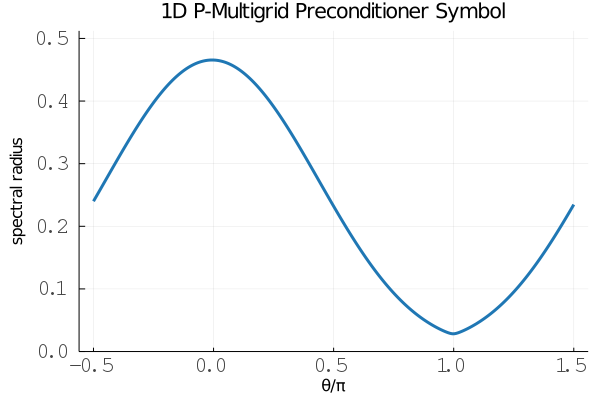
\includegraphics[width=0.48\textwidth]{../img/pmultigridSymbol1D}\label{fig:p_multigrid_spectrum_1d}}
  \hfill
  \subfloat[Spectrum of P-Multigrid for $p_f = 4$, $p_c = 2$]{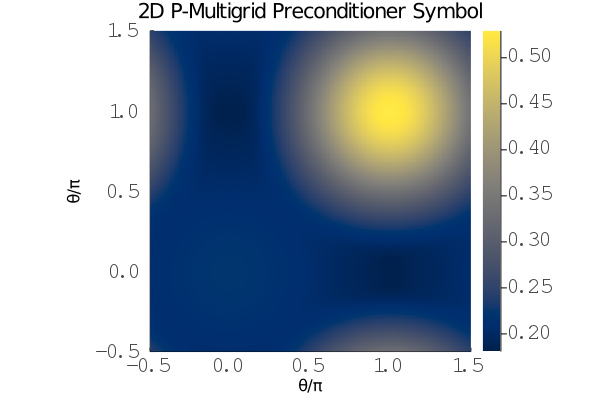
\includegraphics[width=0.48\textwidth]{../img/pmultigridSymbol2D}\label{fig:p_multigrid_spectrum_2d}}
  \caption{Spectrum of Spectrum of P-Multigrid Symbol for $p_f = 4$, $p_c = 2$}
\end{figure}

In Figures \ref{fig:p_multigrid_spectrum_1d} and \ref{fig:p_multigrid_spectrum_2d}, we see the spectral radius of the symbol of p-multigrid for the scalar diffusion operator with third-order Chebyshev smoothing on a fine grid with a fourth-order H1 Lagrange finite element basis and a coarse grid with a second-order H1 Lagrange finite element basis on the Gauss-Lobatto points in one and two dimensions.
Various preconditioning techniques will reduce this spectral radius, with different effectiveness in different frequency ranges.

% -----------------------------------------------------------------------------
\subsection{P-Multigrid Numerical Results}
% -----------------------------------------------------------------------------

In this section, we present numerical results for this analysis for the scalar Laplacian in one and two dimensions with H1 Lagrange bases on Gauss-Lobatto points with Gauss-Legendre quadrature.
Next, we validate these results with numerical experiments for the scalar Laplacian in three dimensions.
Lastly, we consider linear elasticity in three dimensions.

% -----------------------------------------------------------------------------
\subsubsection{Scalar Laplacian - 1D Convergence Factors}\label{sec:1dresults}
% -----------------------------------------------------------------------------

% -----------------------------------------------------------------------------
% Jacobi Smoothing
% -----------------------------------------------------------------------------

\begin{figure}[!tbp]
  \centering
    \subfloat[Convergence for $p = 4$ to $p = 2$, $\nu = 1$]{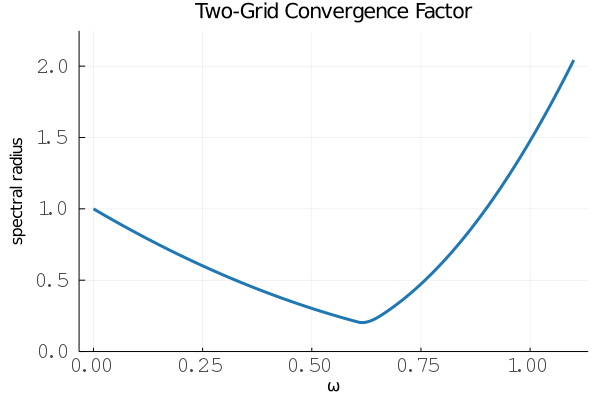
\includegraphics[width=0.48\textwidth]{../img/two_grid_converge_5_to_3}\label{fig:two_grid_5_3}}
    \subfloat[Convergence for $p = 4$ to $p = 1$, $\nu = 1$]{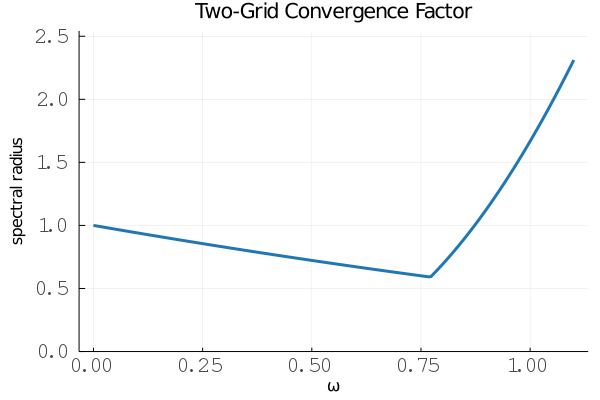
\includegraphics[width=0.48\textwidth]{../img/two_grid_converge_5_to_2}\label{fig:two_grid_5_2}} \\
    \subfloat[Convergence for $p = 4$ to $p = 2$, $\nu = 2$]{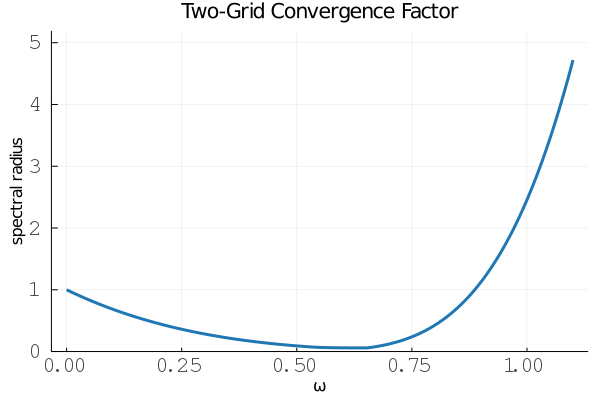
\includegraphics[width=0.48\textwidth]{../img/two_grid_converge_5_to_3_2smooth}\label{fig:two_grid_5_3_2smooth}}
    \subfloat[Convergence for $p = 4$ to $p = 1$, $\nu = 2$]{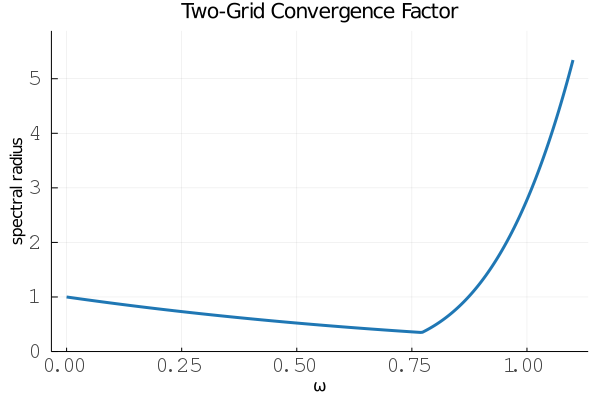
\includegraphics[width=0.48\textwidth]{../img/two_grid_converge_5_to_2_2smooth}\label{fig:two_grid_5_2_2smooth}} \\
  \caption{Two-grid analysis for Jacobi smoothing for high-order finite elements for the 1D Laplacian}
\end{figure}

In Figure \ref{fig:two_grid_5_3} and Figure \ref{fig:two_grid_5_2} we plot the two-grid convergence factor for p-multigrid with a single iteration of Jacobi pre and post-smoothing for the one dimensional Laplacian as a function of the Jacobi smoothing parameter $\omega$,
and in Figure \ref{fig:two_grid_5_3_2smooth} and Figure \ref{fig:two_grid_5_2_2smooth} we plot the two-grid convergence factor for p-multigrid with two iterations of Jacobi pre and post-smoothing for the one dimensional Laplacian as a function of the Jacobi smoothing parameter $\omega$.
On the left we show conservative coarsening from quartic to quadratic elements and on the right we show more aggressive coarsening from quartic to linear elements.
As expected, the two-grid convergence factor decreases as we coarsen more rapidly.
Also, the effect of underestimating the optimal Jacobi smoothing parameter, $\omega$, is less pronounced than the effect of overestimating the smoothing parameter, especially with a higher number of pre and post-smooths.

In contrast to the previous work on h-multigrid for high-order finite elements, \cite{he2020two}, poorly chosen values of $\omega < 1.0$ can result in a spectral radius of the p-multigrid error propagation symbol that is greater than $1$, indicating that application of p-multigrid with Jacobi smoothing at these parameter values will result in increased error.

\begin{table}[ht!]
\begin{center}
\begin{tabular}{l c c c c}
  \toprule
  $p$       &  $\omega_{\min}$  &  $\rho_{\min}$  &  $\omega_{\text{classical}}$  &  $\omega_{\text{highorder}}$  \\
  %\cmidrule(lr){2-3} \cmidrule(lr){4-5} \cmidrule(lr){6-7}
  \midrule
  $p = 2$   &  1.00  &  0.756  & 1.000  &  0.838  \\
  $p = 4$   &  0.91  &  0.955  & 0.911  &  0.855  \\
  $p = 8$   &  0.82  &  0.992  & 0.824  &  0.807  \\
  $p = 16$  &  0.75  &  0.998  & 0.752  &  0.749  \\
  \bottomrule
\end{tabular}
\end{center}
\caption{Jacobi smoothing factor for 1D Laplacian}
\label{table:smoothing_factor_1d_jacobi}
\end{table}

\begin{table}[ht!]
\begin{center}
\begin{tabular}{l cc cc cc}
  \toprule
  $p_{\text{fine}}$ to $p_{\text{coarse}}$  &  \multicolumn{2}{c}{$\nu = 1$}  &  \multicolumn{2}{c}{$\nu = 2$}  &  \multicolumn{2}{c}{$\nu = 3$}  \\
  %\cmidrule(lr){2-3} \cmidrule(lr){4-5} \cmidrule(lr){6-7}
                       &  $\rho_{\min}$ & $\omega_{\text{opt}}$  &  $\rho_{\min}$ & $\omega_{\text{opt}}$  &  $\rho_{\min}$ & $\omega_{\text{opt}}$  \\
  \toprule
  $p = 2$ to $p = 1$   &  0.137 & 0.63  &  0.060 & 0.69  &  0.041 & 0.72   \\
  \midrule
  $p = 4$ to $p = 2$   &  0.204 & 0.62  &  0.059 & 0.64  &  0.045 & 0.70   \\
  $p = 4$ to $p = 1$   &  0.591 & 0.77  &  0.350 & 0.77  &  0.207 & 0.77   \\
  \midrule
  $p = 8$ to $p = 4$   &  0.250 & 0.60  &  0.068 & 0.60  &  0.033 & 0.63   \\
  $p = 8$ to $p = 2$   &  0.668 & 0.73  &  0.446 & 0.73  &  0.298 & 0.73   \\
  $p = 8$ to $p = 1$   &  0.874 & 0.78  &  0.764 & 0.78  &  0.668 & 0.78   \\
  \midrule
  $p = 16$ to $p = 8$  &  0.300 & 0.57  &  0.090 & 0.57  &  0.035 & 0.58   \\
  $p = 16$ to $p = 4$  &  0.719 & 0.69  &  0.517 & 0.69  &  0.371 & 0.69   \\
  $p = 16$ to $p = 2$  &  0.906 & 0.73  &  0.820 & 0.73  &  0.743 & 0.73   \\
  $p = 16$ to $p = 1$  &  0.968 & 0.74  &  0.936 & 0.74  &  0.906 & 0.74   \\
  \bottomrule
\end{tabular}
\end{center}
\caption{Two-grid convergence factor and optimal Jacobi parameter for the 1D Laplacian}
\label{table:two_grid_1d}
\end{table}

The results in Table \ref{table:two_grid_1d} provide the LFA convergence factor and optimal values of $\omega$ for two-grid high-order p-multigrid for a variety of polynomial orders and coarsening factors.

For low order h-multigrid, the classical estimate of the optimal Jacobi smoothing parameter is given by $\omega = 2 / \left( \lambda_{\text{max, high}} + \lambda_{\text{min, high}} \right)$, where $\lambda_{\text{max, high}}$ and $\lambda_{\text{min, high}}$ are the maximum and minimum eigenvalues of $\tilde{S}_f \left( \boldsymbol{\theta} \right)$ for $\boldsymbol{\theta} \in T^{\text{high}}$.
The modified estimate from \cite{he2020two} for h-multigrid for high-order finite elements is given by $\omega = 2 / \left( \lambda_{\text{max}} + \lambda_{\text{min, high}} \right)$, where $\lambda_{\text{max}}$ is the maximum eigenvalue of $\tilde{S}_f \left( \boldsymbol{\theta} \right)$ for $\boldsymbol{\theta} \in T^{\text{low}} \cup T^{\text{high}}$.

In Table \ref{table:smoothing_factor_1d_jacobi} we compare the value of $\omega$ that results in the smallest Jacobi smoothing factor, $\omega_{\min}$, the value given by the classical estimate $\omega_{\text{classical}}$, and the high-order h-multigrid value given by \cite{he2020two}, $\omega_{\text{highorder}}$.
The classical and high-order h-multigrid estimates of the optimal smoothing parameter closely agree as $p$ increases, however these values all overestimate the true optimal smoothing parameter value.

The high-order h-multigrid estimate for $\omega$ provides the best estimate of the optimal value of $\omega$ for two-grid convergence; however, this estimate still overestimates the true optimal smoothing parameter and the quality of this estimate degrades as $p$ increases.

Optimal parameter estimation is an open question for high-order p-multigrid, but optimization techniques, such as those discussed in \cite{brown2021tuning}, can be used to tune these parameters, especially for more complex PDEs.

% -----------------------------------------------------------------------------
% Chebyshev Smoothing
% -----------------------------------------------------------------------------

\begin{figure}[!tbp]
  \centering
    \subfloat[Convergence for $p = 4$ to $p = 2$, $\nu = 1$]{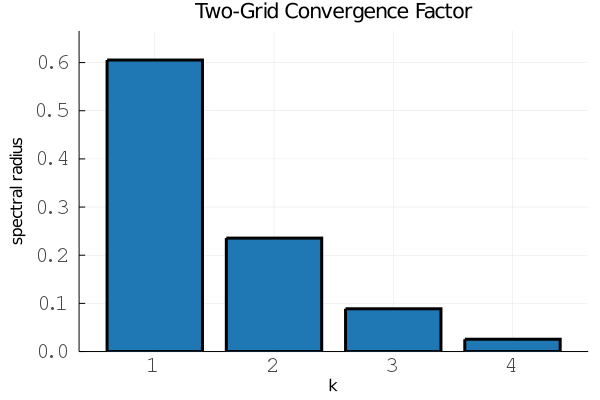
\includegraphics[width=0.48\textwidth]{../img/two_grid_converge_5_to_3_chebyshev}\label{fig:two_grid_5_3_chebyshev}}
    \subfloat[Convergence for $p = 4$ to $p = 1$, $\nu = 1$]{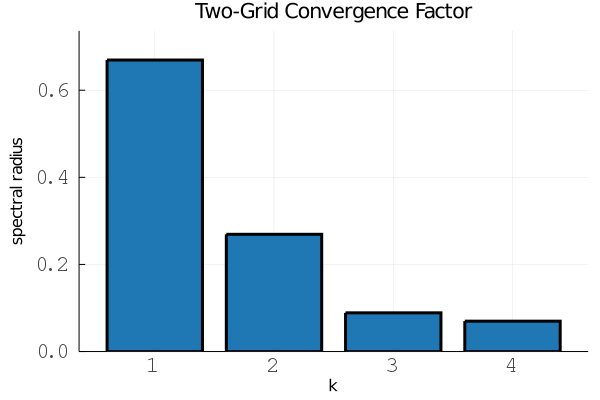
\includegraphics[width=0.48\textwidth]{../img/two_grid_converge_5_to_2_chebyshev}\label{fig:two_grid_5_2_chebyshev}}
  \caption{Two-grid analysis for Chebyshev smoothing for high-order finite elements for the 1D Laplacian}
\end{figure}

In Figure \ref{fig:two_grid_5_3_chebyshev} and Figure \ref{fig:two_grid_5_2_chebyshev} we plot the two-grid convergence factor for p-multigrid with Chebyshev pre and post-smoothing for the one dimensional Laplacian as a function of the Chebyshev order, $k$.
On the left we show conservative coarsening from quartic to quadratic elements and on the right we show more aggressive coarsening from quartic to linear elements.
As expected, the two-grid convergence factor decreases as we coarsen more rapidly.

\begin{table}[ht!]
\begin{center}
\begin{tabular}{l c c c c}
  \toprule
  $p_{\text{fine}}$ to $p_{\text{coarse}}$  &  $k = 1$   &  $k = 2$   &  $k = 3$   &  $k = 4$   \\
  %\cmidrule(lr){2-3} \cmidrule(lr){4-5} \cmidrule(lr){6-7}
  \toprule
  $p = 2$ to $p = 1$   &  0.545  &  0.220  &  0.063  &  0.017  \\
  \midrule
  $p = 4$ to $p = 2$   &  0.576  &  0.222  &  0.089  &  0.025  \\
  $p = 4$ to $p = 1$   &  0.623  &  0.269  &  0.089  &  0.070  \\
  \midrule
  $p = 8$ to $p = 4$   &  0.638  &  0.244  &  0.074  &  0.022  \\
  $p = 8$ to $p = 2$   &  0.657  &  0.260  &  0.097  &  0.059  \\
  $p = 8$ to $p = 1$   &  0.881  &  0.674  &  0.510  &  0.393  \\
  \midrule
  $p = 16$ to $p = 8$  &  0.664  &  0.253  &  0.075  &  0.022  \\
  $p = 16$ to $p = 4$  &  0.714  &  0.328  &  0.135  &  0.059  \\
  $p = 16$ to $p = 2$  &  0.907  &  0.741  &  0.602  &  0.496  \\
  $p = 16$ to $p = 1$  &  0.970  &  0.912  &  0.857  &  0.809  \\
  \bottomrule
\end{tabular}
\end{center}
\caption{Two-grid convergence factor with Chebyshev smoothing for 1D Laplacian}
\label{table:two_grid_1d_chebyshev}
\end{table}

The results in Table \ref{table:two_grid_1d_chebyshev} provide the LFA convergence factor and optimal values of $k$ for two-grid high-order p-multigrid for a variety of coarsening rates and orders of Chebyshev smoother.
From this table, we can see that the effectiveness of higher order Chebyshev smoothers degrades as we coarsen more aggressively, but Chebyshev smoothing still provides better two-grid convergence than multiple pre and post-smoothing Jacobi iterations.

% -----------------------------------------------------------------------------
\subsubsection{Scalar Laplacian - 2D Convergence Factors}\label{sec:2dresults}
% -----------------------------------------------------------------------------

% -----------------------------------------------------------------------------
% Jacobi Smoothing
% -----------------------------------------------------------------------------

In Figure \ref{fig:jacobi_smooth_factor_2d} and Figure \ref{fig:two_grid_5_to_3_2d} we show the Jacobi smoothing factor and two-grid convergence factor for p-multigrid with one iteration of Jacobi smoothing for the two dimensional Laplacian as a function of the Jacobi smoothing parameter $\omega$, while Table \ref{table:smoothing_factor_2d_jacobi} shows estimates of optimal the Jacobi smoothing factor for two-grid convergence.
These values generally fail to accurately estimate the true optimal smoothing parameter value, again providing over-estimates to the true optimal smoothing parameter in most cases.

\begin{figure}[!tbp]
  \centering
  \subfloat[Smoothing Factor of 2D Jacobi for $p = 4$, $\nu = 1$]{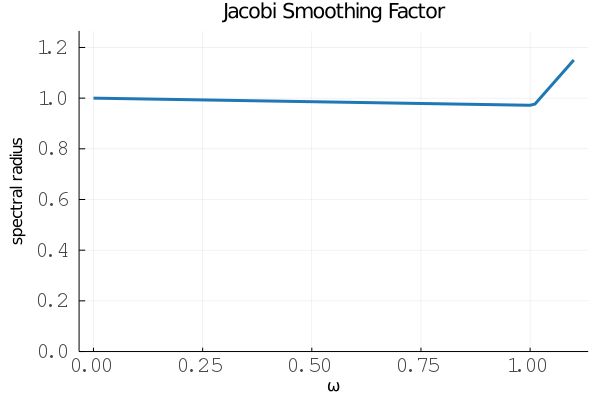
\includegraphics[width=0.48\textwidth]{../img/jacobi_smoothing_5_2d}\label{fig:jacobi_smooth_factor_2d}}
  \hfill
  \subfloat[Convergence for $p = 4$ to $p = 2$, $\nu = 1$]{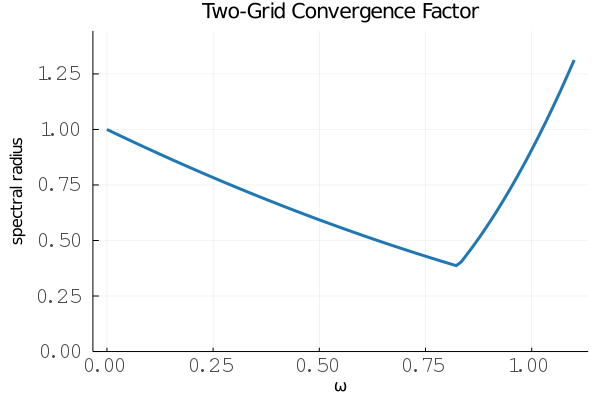
\includegraphics[width=0.48\textwidth]{../img/two_grid_converge_5_to_3_2d}\label{fig:two_grid_5_to_3_2d}}
  \caption{Convergence for high-order finite elements for the 2D Laplacian}
\end{figure}

\begin{table}[ht!]
\begin{center}
\begin{tabular}{l c c c c}
  \toprule
  $p$       &  $\omega_{\min}$  &  $\rho_{\min}$  &  $\omega_{\text{classical}}$  &  $\omega_{\text{highorder}}$  \\
  %\cmidrule(lr){2-3} \cmidrule(lr){4-5} \cmidrule(lr){6-7}
  \midrule
  $p = 2$   &  1.05  &  0.839  & 1.218  &  1.173  \\
  $p = 4$   &  1.00  &  0.972  & 1.009  &  1.001  \\
  $p = 8$   &  0.87  &  0.955  & 0.880  &  0.880  \\
  \bottomrule
\end{tabular}
\end{center}
\caption{Jacobi smoothing factor for 2D Laplacian}
\label{table:smoothing_factor_2d_jacobi}
\end{table}

\begin{table}[ht!]
\begin{center}
\begin{tabular}{l cc cc cc}
  \toprule
  $p_{\text{fine}}$ to $p_{\text{coarse}}$  &  \multicolumn{2}{c}{$\nu = 1$}  &  \multicolumn{2}{c}{$\nu = 2$}  &  \multicolumn{2}{c}{$\nu = 3$}  \\
  %\cmidrule(lr){2-3} \cmidrule(lr){4-5} \cmidrule(lr){6-7}
                      &  $\rho_{\min}$  &  $\omega_{\text{opt}}$  &  $\rho_{\min}$ & $\omega_{\text{opt}}$  &  $\rho_{\min}$ & $\omega_{\text{opt}}$  \\
  \toprule
  $p = 2$ to $p = 1$  &  0.230 & 0.95  &  0.091 & 0.99  &  0.061 & 1.03   \\
  \midrule
  $p = 4$ to $p = 2$  &  0.388 & 0.82  &  0.151 & 0.82  &  0.078 & 0.83   \\
  $p = 4$ to $p = 1$  &  0.763 & 0.95  &  0.582 & 0.95  &  0.444 & 0.95   \\
  \midrule
  $p = 8$ to $p = 4$  &  0.646 & 0.79  &  0.418 & 0.79  &  0.272 & 0.79   \\
  $p = 8$ to $p = 2$  &  0.858 & 0.84  &  0.737 & 0.84  &  0.633 & 0.84   \\
  $p = 8$ to $p = 1$  &  0.952 & 0.87  &  0.907 & 0.87  &  0.864 & 0.87   \\
  \bottomrule
\end{tabular}
\end{center}
\caption{Two-grid convergence factor and optimal Jacobi parameter for 2D Laplacian}
\label{table:two_grid_2d}
\end{table}

The results in Table \ref{table:two_grid_2d} provide the LFA convergence factor and optimal values of $\omega$ for two-grid high-order p-multigrid for a variety of polynomial orders and coarsening factors.

% -----------------------------------------------------------------------------
% Chebyshev Smoothing
% -----------------------------------------------------------------------------

\begin{table}[ht!]
\begin{center}
\begin{tabular}{l c c c c}
  \toprule
  $p_{\text{fine}}$ to $p_{\text{coarse}}$  &  $k = 1$   &  $k = 2$   &  $k = 3$   &  $k = 4$   \\
  %\cmidrule(lr){2-3} \cmidrule(lr){4-5} \cmidrule(lr){6-7}
  \toprule
  $p = 2$ to $p = 1$   &  0.621  &  0.252  &  0.075  &  0.039  \\
  \midrule
  $p = 4$ to $p = 2$   &  0.607  &  0.281  &  0.085  &  0.047  \\
  $p = 4$ to $p = 1$   &  0.768  &  0.424  &  0.219  &  0.127  \\
  \midrule
  $p = 8$ to $p = 4$   &  0.669  &  0.278  &  0.110  &  0.055  \\
  $p = 8$ to $p = 2$   &  0.864  &  0.633  &  0.456  &  0.336  \\
  $p = 8$ to $p = 1$   &  0.956  &  0.873  &  0.795  &  0.730  \\
  \midrule
  $p = 16$ to $p = 8$  &  0.855  &  0.613  &  0.435  &  0.319  \\
  $p = 16$ to $p = 4$  &  0.938  &  0.822  &  0.719  &  0.634  \\
  $p = 16$ to $p = 2$  &  0.976  &  0.928  &  0.882  &  0.842  \\
  $p = 16$ to $p = 1$  &  0.992  &  0.975  &  0.959  &  0.944  \\
  \bottomrule
\end{tabular}
\end{center}
\caption{Two-grid convergence factor with Chebyshev smoothing for 2D Laplacian}
\label{table:two_grid_2d_chebyshev}
\end{table}

The results in Table \ref{table:two_grid_2d_chebyshev} provide the LFA convergence factor and optimal values of $k$ for two-grid high-order p-multigrid for a variety of coarsening rates and orders of Chebyshev smoother.
The two-grid convergence factor still degrades and the effectiveness of higher order Chebyshev smoothers is again reduced as we coarsen more aggressively.

% -----------------------------------------------------------------------------
\subsubsection{Scalar Laplacian - 3D Convergence Factors}\label{sec:3dresults}
% -----------------------------------------------------------------------------

In this section, we compare the LFA two-grid convergence factors to numerical results.
Our numerical experiments were conducted using the libCEED \cite{libceed-user-manual} with PETSc \cite{petsc-user-ref} multigrid example found in the libCEED repository.
PETSc provides the mesh management, linear solvers, and multigrid preconditioner while libCEED provides the matrix-free operator evaluation.

We recover the manufactured solution given by
\begin{equation}
f \left( x, y, z \right) = x y z \sin \left( \pi x \right) \sin \left( \pi \left( 1.23 + 0.5 y \right) \right) \sin \left( \pi \left( 2.34 + 0.25 z \right) \right)
\end{equation}
on the domain $\left[ -3, 3 \right]^3$ with approximately 8 million degrees of freedom for a variety of test cases.
Although LFA is define on infinite grids, which most naturally translate to periodic problems, LFA predicted convergence factors are also accurate for appropriate problems with other boundary conditions on finite grids \cite{rodrigo2019validity}.

% -----------------------------------------------------------------------------
% Jacobi Smoothing
% -----------------------------------------------------------------------------

Since the Chebyshev smoothing is based upon the Jacobi preconditioned operator, it is important to validate the LFA of the Jacobi smoothing before considering Chebyshev smoothing.
We use simple Jacobi smoothing with a weight of $\omega = 1.0$ to validate the LFA.

\begin{table}[ht!]
\begin{center}
\begin{tabular}{l c c}
  \toprule
  $p_{\text{fine}}$ to $p_{\text{coarse}}$  &  LFA  &  libCEED  \\
  %\cmidrule(lr){2-3} \cmidrule(lr){4-5} \cmidrule(lr){6-7}
  \toprule
  $p = 2$ to $p = 1$   &  0.312  &  0.301  \\
  \midrule
  $p = 4$ to $p = 2$   &  1.436  &  1.402  \\
  $p = 4$ to $p = 1$   &  1.436  &  1.401  \\
  \midrule
  $p = 8$ to $p = 4$   &  1.989  &  1.885  \\
  $p = 8$ to $p = 2$   &  1.989  &  1.874  \\
  $p = 8$ to $p = 1$   &  1.989  &  1.875  \\
  \bottomrule
\end{tabular}
\end{center}
\caption{LFA and experimental two-grid convergence factor with Jacobi smoothing for 3D Laplacian with $\omega = 1$}
\label{table:two_grid_3d_jacobi}
\end{table}

The results in Table \ref{table:two_grid_3d_jacobi} provide the LFA and experimental convergence factors for the test problem.
As expected, the high-order fine grid problems diverge with a smoothing factor of $\omega = 1$; however, the LFA provides reasonable upper bounds on the true convergence factor seen in the experimental results.

% -----------------------------------------------------------------------------
% Chebyshev Smoothing
% -----------------------------------------------------------------------------

We used the LFA estimates of the maximal eigenvalue to set the extremal eigenvalues used the Chebyshev iteration in PETSc, using $\lambda_{\text{min}} = 0.1 \hat{\lambda}_{\text{max}}$ and $\lambda_{\text{max}} = 1.0 \hat{\lambda}_{\text{max}}$, where $\hat{\lambda}_{\text{max}}$ is the estimated maximal eigenvalue of the symbol of the Jacobi preconditioned operator.

\begin{table}[ht!]
\begin{center}
\begin{tabular}{l cc cc cc}
  \toprule
  $p_{\text{fine}}$ to $p_{\text{coarse}}$  &  \multicolumn{2}{c}{$k = 2$}  &  \multicolumn{2}{c}{$k = 3$}  &  \multicolumn{2}{c}{$k = 4$}  \\
  %\cmidrule(lr){2-3} \cmidrule(lr){4-5} \cmidrule(lr){6-7}
                      &  LFA  &  libCEED  &  LFA  &  libCEED  &  LFA  &  libCEED  \\
  \toprule
  $p = 2$ to $p = 1$  &  0.253 & 0.222  &  0.076 & 0.058  &  0.041 & 0.033  \\
  \midrule
  $p = 4$ to $p = 2$  &  0.277 & 0.251  &  0.111 & 0.097  &  0.062 & 0.050  \\
  $p = 4$ to $p = 1$  &  0.601 & 0.587  &  0.416 & 0.398  &  0.295 & 0.276  \\
  \midrule
  $p = 8$ to $p = 4$  &  0.398 & 0.391  &  0.197 & 0.195  &  0.121 & 0.110  \\
  $p = 8$ to $p = 2$  &  0.748 & 0.743  &  0.611 & 0.603  &  0.506 & 0.469  \\
  $p = 8$ to $p = 1$  &  0.920 & 0.914  &  0.871 & 0.861  &  0.827 & 0.814  \\
  \bottomrule
\end{tabular}
\end{center}
\caption{LFA and experimental two-grid convergence factor with Chebyshev smoothing for 3D Laplacian}
\label{table:two_grid_3d_chebyshev}
\end{table}

The LFA provides reasonable upper bounds on the true convergence factor seen in the experimental results.
As with the one and two dimensional results, rapid coarsening of the polynomial order of the bases decreases the effectiveness of higher order Chebyshev smoothing.

% -----------------------------------------------------------------------------
\subsubsection{Linear Elasticity - 3D Convergence Factors}\label{sec:solidsresults}
% -----------------------------------------------------------------------------

To demonstrate the suitability of this LFA formulation for more complex PDE, we consider linear elasticity in three dimensions.
The strong form of the static balance of linear momentum at small strain for the three dimensional linear elasticity problem is given by \cite{hughes2012finite} as
\begin{equation}
\nabla \cdot \boldsymbol{\sigma} + \boldsymbol{g} = \boldsymbol{0}
\end{equation}
where $\boldsymbol{\sigma}$ is the stress function and $\boldsymbol{g}$ is the forcing function.
This strong form has the corresponding weak form
\begin{equation}
\int_{\Omega} \nabla \mathbf{v} : \boldsymbol{\sigma} dV - \int_{\partial \Omega} \mathbf{v} \cdot \left( \boldsymbol{\sigma} \cdot \hat{\mathbf{n}} \right) dS - \int_{\Omega} \mathbf{v} \cdot \mathbf{g} dV = 0, \forall \mathbf{v} \in \mathcal{V}
\end{equation}
for some displacement $\mathbf{u} \in \mathcal{V} \subset H^1 \left( \Omega \right)$, where $:$ denotes contraction over both components and dimensions.

Linear elasticity constitutive modeling is based upon the Lamé parameters,
\begin{equation}
\begin{split}
\lambda & = \frac{E \nu}{\left( 1 + \nu \right) \left( 1 - 2 \nu \right)} \\
\mu & = \frac{E}{2 \left( 1 + \nu \right)}
\end{split}
\end{equation}
where $E$ is the Young's modulus and $\nu$ is the Poisson's ratio for the materiel.

In the linear elasticity constitutive model, the symmetric strain tensor is given by
\begin{equation}
\boldsymbol{\epsilon} = \frac{1}{2} \left( \nabla \mathbf{u} + \nabla \mathbf{u}^T \right)
\end{equation}
and the linear elasticity constitutive law is given by $\boldsymbol{\sigma} = \mathsf{C} : \boldsymbol{\epsilon}$ where
\begin{equation}
\mathsf{C} =
\begin{bmatrix}
   \lambda + 2\mu & \lambda & \lambda & & & \\
   \lambda & \lambda + 2\mu & \lambda & & & \\
   \lambda & \lambda & \lambda + 2\mu & & & \\
   & & & \mu & & \\
   & & & & \mu & \\
   & & & & & \mu
\end{bmatrix}.
\end{equation}

\begin{table}[ht!]
\begin{center}
\begin{tabular}{l c c c c}
  \toprule
  $p_{\text{fine}}$ to $p_{\text{coarse}}$  &  $k = 1$   &  $k = 2$   &  $k = 3$   &  $k = 4$   \\
  %\cmidrule(lr){2-3} \cmidrule(lr){4-5} \cmidrule(lr){6-7}
  \toprule
  $p = 2$ to $p = 1$   &  0.621  &  0.252  &  0.075  &  0.039  \\
  \midrule
  $p = 4$ to $p = 2$   &  0.607  &  0.281  &  0.085  &  0.047  \\
  $p = 4$ to $p = 1$   &  0.768  &  0.424  &  0.219  &  0.127  \\
  \midrule
  $p = 8$ to $p = 4$   &  0.669  &  0.278  &  0.110  &  0.055  \\
  $p = 8$ to $p = 2$   &  0.864  &  0.633  &  0.456  &  0.336  \\
  $p = 8$ to $p = 1$   &  0.956  &  0.873  &  0.795  &  0.730  \\
  \bottomrule
\end{tabular}
\end{center}
\caption{Two-grid convergence factor with Chebyshev smoothing for 3D linear elasticity}
\label{table:two_grid_3d_linear_elasticity}
\end{table}

The results in Table \ref{table:two_grid_3d_linear_elasticity} provide the LFA convergence factor and optimal values of $k$ for two-grid high-order p-multigrid for a variety of coarsening rates and orders of Chebyshev smoother.
